\documentclass{iagtese} 		% declaração da classe iagtese com
						% padrões de formatação.
						%	
%\documentclass{iagtese_en}	% declaração da classe iagtese em
						% ingles. Para escrever a tese em 
						% ingles, descomente esta linha e 
						% comente a linha anterior.
						%				%	
%\hypercolor				% links coloridos para a versao
						% on line da tese. Para usar esta
						% opcao descomente esta linha.
						% 	
\begin{document}			% início do documento
						% 				
\institution{Universidade de São Paulo \\ Instituto de Astronomia, Geofísica e Ciências Atmosféricas \\ Departamento de Astronomia}

\title{Título do trabalho}

\translator{{Tese/Dissertação apresentada ao Departamento de Astronomia do Instituto de Astronomia, Geofísica e Ciências Atmosféricas da Universidade de São Paulo como requisito parcial para a obtenção do título de Mestre/{}Doutor em Ciências.\\ \\
Área de Concentração: Astronomia\\
Orientador(a): Prof.($^{\rm a}$) Dr.($^{\rm a}$) Orientador(a)}}

\author{Autor}

\date{São Paulo \ano}			% arquivo para inserir a capa
						%
\pagestyle{empty}			% padrão de formatação para parte
						% inicial do texto
						%
\maketitle					% 
						%
\Dedicatoria				%
\hfill
\vfill
\hfill{\it{sua dedicatoria aqui!}}
\vspace{2cm}		%
						% componentes iniciais do trabalho
\Agradecimentos			%
À minha família;

À fulana;

À orientadora;

Aos pesquisadores;

À Professora;

Aos colegas: 1, 2, 3 e 4

À FAPESP, pelo apoio financeiro, sob o projeto n$^o$: 6666/6666;

Às Instituições

\vfill

\begin{flushleft}
\rule{6cm}{0.5pt}\\
{\footnotesize{Esta tese/dissertação foi escrita em \LaTeX{} com a classe IAGTESE, para teses e dissertações do IAG.}}
\end{flushleft}	% caso não queira adicionar algum
						% deles, simplesmente remova as
						% linhas correspondentes.
						%
\Epigrafe					%  
\vfill
\begin{flushright}

``\textit{frase bonita 01}''\\

\vspace{0.4cm}

Autor da frase bonita 01

\end{flushright}

\vspace{0.5cm}

\begin{flushright}

``\textit{frase bonita 02}''\\

\vspace{0.4cm}

Autor da frase bonita 02

\end{flushright}

\vspace{2cm}		%
						%
\Resumo					%
Resumo		%
						%
\Abstract					%
% ---
% RESUMOS
% ---

% resumo em português
\setlength{\absparsep}{18pt} % ajusta o espaçamento dos parágrafos do resumo
\begin{resumo}
 ...

 \textbf{Palavras-chave}: ...
\end{resumo}

% resumo em inglês
\begin{resumo}[Abstract]
 \begin{otherlanguage*}{english}
   ...

   \vspace{\onelineskip}
 
   \noindent 
   \textbf{Keywords}: ...
 \end{otherlanguage*}
\end{resumo}		%
						%
\listoffigures 				% lista de figuras (opcional)
\listoftables 				% lista de tabelas (opcional)
\tableofcontents 			% sumário
						%
\cleardoublepage			%
\pagestyle{fancy}			% formatação para corpo do texto
						%
\chapter{Introdução}
\label{intro}

\section{como incluir citações utilizando bibTeX}

\begin{verbatim}O comando \citet{doutorado} produz:\end{verbatim}
\citet{doutorado}

\begin{verbatim}O comando \citet{mestrado} produz:\end{verbatim}
\citet{mestrado}

\begin{verbatim}O comando \citet*{artigo1} produz:\end{verbatim}
\citet*{artigo1}

\begin{verbatim}O comando \citet{artigo2} produz:\end{verbatim}
\citet{artigo2}

\begin{verbatim}O comando \citet{bethe} produz:\end{verbatim}
\citet{bethe}

\begin{verbatim}O comando \citet{livro} produz:\end{verbatim}
\citet{livro}

\begin{verbatim}O comando \citet{feynman} produz:\end{verbatim}
\citet{feynman}

\begin{verbatim}O comando \cite{salpeter} produz:\end{verbatim}
\cite{salpeter}

\section{próxima seção}

\subsection{subseção}

\subsubsection{subsubseção}

\paragraph{parágrafo}		%
\chapter{Base de dados}\label{database}

Base de dados. Citar figura \ref{identificador}.

\begin{figure}[!ht]
\begin{center}
\setcaptionmargin{1cm}
\includegraphics[width=1.0 \columnwidth,angle=0]{fig/solar_grevesse.eps}
\caption[Resumo da legenda da figura (aparece na lista de figuras)]{Legenda da figura.} 
\label{identificador}
\end{center}
\end{figure}


\begin{center}
\setcaptionmargin{1cm}
\scriptsize
\begin{longtable}{lcccc}
\caption[Resumo da legenda da tabela (aparece na lista de figuras)]{Exemplo de tabela feita com o longtable.}\\
\hline \hline \\[-2ex]
\multicolumn{1}{c}{Coluna1} &
\multicolumn{1}{c}{Coluna2} &
\multicolumn{1}{c}{Coluna3} &
\multicolumn{1}{c}{Coluna4} &
\multicolumn{1}{c}{Coluna5} 

\\[0.5ex] \hline
\\[-1.8ex]

\endfirsthead

\multicolumn{5}{c}{\footnotesize{{\slshape{{\tablename} \thetable{}}} - Continuação}}\\[0.5ex]

\hline \hline\\[-2ex]

\multicolumn{1}{c}{Coluna1} &
\multicolumn{1}{c}{Coluna2} &
\multicolumn{1}{c}{Coluna3} &
\multicolumn{1}{c}{Coluna4} &
\multicolumn{1}{c}{Coluna5} 

\\[0.5ex] \hline
\\[-1.8ex]

\endhead

\multicolumn{3}{l}{{\footnotesize{Continua na próxima página\ldots}}}\\
\endfoot
\hline

\endlastfoot

1 & 2 & 3 & 4 & 5 \\
6 & 7 & 8 & 9 & 10\\

\label{tabela_com_longtable}
\end{longtable}
\end{center}    	% inserir os capítulos do seu
\chapter{Análise}


Análise		% trabalho.
\chapter{Conclusões}\label{conc}

Conclusões do trabalho e/{}ou perspectivas		% 
       						%
						%
%\begin{thebibliography}{99}	% referências bibliográficas (dê
%\bibitem{Quireza et al. 2007}{quireza}Quireza C., Rocha-Pinto H. J., Maciel W. J., 2007, A\&A, 475, 217

\bibitem[Aoki et al.(2001)]{2001ApJ...561..346A} Aoki, W., Ryan, S. G., Norris, J. E., Beers, T. C., Ando, H., Iwamoto, N., Kajino, T., Mathews, G. J., \& Fujimoto, M. Y. 2001, ApJ 561, 346

\bibitem[Aoki et al.(2002)]{2002ApJ...580.1149A} Aoki, W., Ryan, S. G., Norris, J. E., Beers, T. C., Ando, H., \& Tsangarides, S. 2002, ApJ 580, 1149 

\bibitem[Wasserburg et al. (1994)]{1994ApJ...424..412W} Wasserburg, G. J., Busso, M., Gallino, R., \& Raiteri, C. M. 1994, ApJ 424, 412 	% preferência ao bibTeX).
%\end{thebibliography}		% caso não use o bibTeX, remova os
						% comentarios das três linhas
						% e comente a linha \bibliography
						%
\bibliography{tex/bibliografia}	% bibliografia utilizando bibTeX,
						% referente ao arquivo
						% bibliografia.bib na pasta tex/
						%
\begin{apendice}			% inicio do ambiente apendice
\chapter{título do apêndice 01}\label{ap01}

\section{subtítulo 01}\label{subap01}

\chapter{título do apêndice 02}\label{ap02}		% texto referente ao apendice
\end{apendice}				% fim do ambiente apendice. caso
						% nao utilize apendice, remova as
						% 3 linhas de comando.
						%
\end{document}				% fim do arquivo